\documentclass[aspectratio=169,10pt]{beamer}

% -----------------------------------------------------------------------------
% Theme and Color Styling
% -----------------------------------------------------------------------------
\usetheme{Madrid}
\usecolortheme{whale}

% Modern corporate/academic color palette
\definecolor{NavyBlue}{RGB}{15, 37, 75}
\definecolor{TealAccent}{RGB}{13, 148, 136}
\definecolor{SlateGray}{RGB}{100, 116, 139}
\definecolor{LightBg}{RGB}{248, 250, 252}
\definecolor{AlertRed}{RGB}{225, 29, 72}
\definecolor{SuccessGreen}{RGB}{16, 185, 129}
\definecolor{WarmAmber}{RGB}{217, 119, 6}
\definecolor{amber}{RGB}{217, 119, 6}

\setbeamercolor{palette primary}{bg=NavyBlue, fg=white}
\setbeamercolor{palette secondary}{bg=NavyBlue!85, fg=white}
\setbeamercolor{palette tertiary}{bg=NavyBlue!70, fg=white}
\setbeamercolor{titlelike}{bg=NavyBlue, fg=white}
\setbeamercolor{frametitle}{bg=NavyBlue, fg=white}
\setbeamercolor{structure}{fg=NavyBlue}
\setbeamercolor{block title}{bg=NavyBlue, fg=white}
\setbeamercolor{block body}{bg=LightBg, fg=black}
\setbeamercolor{block title alerted}{bg=AlertRed, fg=white}
\setbeamercolor{block body alerted}{bg=AlertRed!10, fg=black}
\setbeamercolor{block title example}{bg=TealAccent, fg=white}
\setbeamercolor{block body example}{bg=TealAccent!10, fg=black}

% Customize footline
\setbeamertemplate{navigation symbols}{}
\setbeamertemplate{footline}{
  \leavevmode%
  \hbox{%
  \begin{beamercolorbox}[wd=.333333\paperwidth,ht=2.25ex,dp=1ex,center]{author in head/foot}%
    \usebeamerfont{author in head/foot}P. Bhat, S. Kumar, H. Mehar
  \end{beamercolorbox}%
  \begin{beamercolorbox}[wd=.333333\paperwidth,ht=2.25ex,dp=1ex,center]{title in head/foot}%
    \usebeamerfont{title in head/foot}IT488 Large Language Models
  \end{beamercolorbox}%
  \begin{beamercolorbox}[wd=.333333\paperwidth,ht=2.25ex,dp=1ex,right]{date in head/foot}%
    \usebeamerfont{date in head/foot}\insertframenumber{} / \inserttotalframenumber\hspace*{2ex}
  \end{beamercolorbox}}%
  \vskip0pt%
}

% -----------------------------------------------------------------------------
% Required Packages
% -----------------------------------------------------------------------------
\usepackage{amsmath, amssymb}
\usepackage{booktabs}
\usepackage{array}
\usepackage{tikz}
\usetikzlibrary{shapes.geometric, arrows.meta, positioning, calc, shadows}
\usepackage{graphicx}
\usepackage{colortbl}

% -----------------------------------------------------------------------------
% Metadata
% -----------------------------------------------------------------------------
\title[QLoRA Algorithmic Distillation]{\textbf{QLoRA Distillation for Algorithmic Code Classification and Generation}}
\subtitle{Addressing the ``Valley of Code Reasoning'' via Decoupled Algorithmic Conditioning}
\author[P. Bhat, S. Kumar, H. Mehar]{
  \textbf{Pranav Bhat P} (231IT049) \quad
  \textbf{Shivam Kumar} (231IT068) \quad
  \textbf{Himanshu Mehar} (231IT027)
}
\institute[NITK Surathkal]{
  \textbf{Course: IT488 -- Large Language Models} \\
  Department of Information Technology \\
  National Institute of Technology Karnataka (NITK), Surathkal
}
\date{Midsemester Evaluation -- March 2026}

% -----------------------------------------------------------------------------
% Document Body
% -----------------------------------------------------------------------------
\begin{document}

% Slide 1: Title Slide
\begin{frame}[plain]
  \titlepage
\end{frame}

% Slide 2: Outline
\begin{frame}{Presentation Outline}
  \tableofcontents
\end{frame}

% =============================================================================
\section{Introduction \& Motivation}
% =============================================================================

\begin{frame}{Base Paper: Findings \& Drawbacks (He et al., 2025)}
  \begin{columns}[T]
    \begin{column}{0.48\textwidth}
      \begin{block}{\textbf{Key Findings of Base Paper}}
        \begin{itemize}\itemsep=2pt\footnotesize
          \item \textbf{The ``Valley of Code Reasoning''}: Intermediate data scaling exhibits a sharp performance dip where student reasoning degrades before recovering.
          \item \textbf{Entangled Token Generation}: Jointly predicting rationale and code forces the model to resolve abstract math and low-level syntax simultaneously.
          \item \textbf{CoT Fragility in Code}: Standard Chain-of-Thought prompts frequently trigger premature convergence to suboptimal brute-force loops ($O(N^2)$).
        \end{itemize}
      \end{block}
    \end{column}

    \begin{column}{0.48\textwidth}
      \begin{alertblock}{\textbf{Critical Drawbacks of Base Paper}}
        \begin{itemize}\itemsep=2pt\footnotesize
          \item \textbf{No Decoupled Planning}: Lacks an explicit System-2 stage to identify the algorithmic paradigm (DP, Graphs, Greedy) before code synthesis.
          \item \textbf{Unfiltered Teacher Contamination}: Assumes teacher rationales are always sound; hallucinated or mismatched traces pollute student supervision.
          \item \textbf{High Compute Dependency}: Evaluated only on multi-billion parameter models ($\ge 7\text{B}$), lacking accessible QLoRA solutions for sub-1B models on consumer GPUs.
        \end{itemize}
      \end{alertblock}
    \end{column}
  \end{columns}

  \vspace{3pt}
  \begin{exampleblock}{Our Approach to Address These Drawbacks}
    \footnotesize
    \textbf{1. Decoupled Algorithmic Conditioning} (Stage 1 Classifier) + \textbf{2. Semantic Rationale Filter} (purging noise) + \textbf{3. Consumer-Grade QLoRA} (Qwen2.5-0.5B on single 15GB T4 GPU).
  \end{exampleblock}
\end{frame}

% =============================================================================
\section{Problem Statement \& Objectives}
% =============================================================================

\begin{frame}{Problem Statement}
  \begin{alertblock}{Core Vulnerabilities in Existing Code Distillation}
    \begin{enumerate}\itemsep=6pt
      \item \textbf{Unstructured Monolithic CoT Generation}: Student models attempt to predict algorithmic intuition and raw syntax simultaneously, leading to hallucinated loops and asymptotic timeout errors ($O(N^2)$ instead of $O(N \log N)$).
      \item \textbf{Teacher Trace Contamination}: Commercial teacher LLMs generate deceptive or mislabeled rationales that diverge from ground-truth paradigms. Distilling noisy traces degrades student reasoning.
      \item \textbf{High Compute Barriers}: Full parameter fine-tuning of multi-billion parameter models is inaccessible to standard edge and consumer hardware.
    \end{enumerate}
  \end{alertblock}
\end{frame}

\begin{frame}{Project Objectives}
  \begin{columns}[T]
    \begin{column}{0.48\textwidth}
      \begin{block}{\textbf{Midsemester Scope (40\%) -- Completed}}
        \begin{itemize}\itemsep=1.5pt\footnotesize
          \item \textbf{100-Problem Benchmark}: Stratified extraction from TACO across 10 algorithmic categories.
          \item \textbf{Teacher Trace Synthesis}: Structured rationales from Gemini 3.5 Flash Lite.
          \item \textbf{Rationale-Consistency Filter}: Automatic semantic verification (82\% retention).
          \item \textbf{Subprocess Sandbox Judge}: Timeout ($2.0\text{s}$) and memory ($512\text{MB}$) isolation.
          \item \textbf{Stage 1 QLoRA Distillation}: Comparative training of HF PEFT vs. Unsloth.
        \end{itemize}
      \end{block}
    \end{column}

    \begin{column}{0.48\textwidth}
      \begin{exampleblock}{\textbf{Endsemester Scope (60\%) -- In Progress}}
        \begin{itemize}\itemsep=1.5pt\footnotesize
          \item \textbf{Stage 2 Conditioned Generator}: Conditioning on $[\text{TAG}] + [\text{PROBLEM}]$ to synthesize $[ \text{RATIONALE} ] + [ \text{CODE} ]$.
          \item \textbf{Empirical Scaling Sweep}: Investigating the ``Valley of Code Reasoning'' across 10\%, 25\%, 50\%, 100\%.
          \item \textbf{Full Pass@k Benchmark}: Sandbox execution judging across all problem suites.
          \item \textbf{Ablation Study}: Conditioned vs. Unconditioned baseline comparison.
        \end{itemize}
      \end{exampleblock}
    \end{column}
  \end{columns}
\end{frame}

% =============================================================================
\section{Methodology \& Architecture}
% =============================================================================

\begin{frame}{Methodology: Decoupled Two-Stage Distillation}
  \begin{center}
  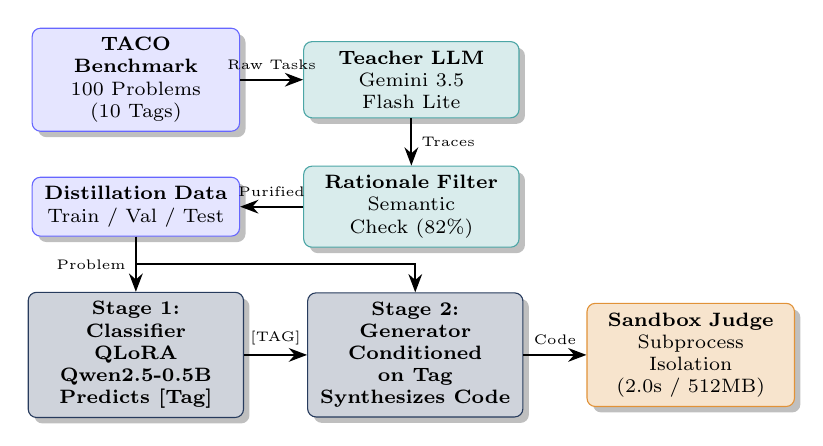
\begin{tikzpicture}[node distance=1.1cm, auto,
    base/.style={draw, rounded corners=3pt, text centered, font=\scriptsize, minimum height=0.65cm, drop shadow},
    data/.style={base, fill=blue!10, draw=blue!60, text width=2.4cm},
    proc/.style={base, fill=teal!15, draw=teal!70, text width=2.5cm},
    model/.style={base, fill=NavyBlue!20, draw=NavyBlue!90, text width=2.5cm, font=\scriptsize\bfseries},
    judge/.style={base, fill=WarmAmber!20, draw=WarmAmber!80, text width=2.4cm}]

    % Nodes
    \node [data] (taco) {\textbf{TACO Benchmark}\\100 Problems (10 Tags)};
    \node [proc, right=0.8cm of taco] (gemini) {\textbf{Teacher LLM}\\Gemini 3.5 Flash Lite};
    \node [proc, below=0.6cm of gemini] (filter) {\textbf{Rationale Filter}\\Semantic Check (82\%)};
    \node [data, left=0.8cm of filter] (clean) {\textbf{Distillation Data}\\Train / Val / Test};
    
    \node [model, below=0.7cm of clean] (stage1) {\textbf{Stage 1: Classifier}\\QLoRA Qwen2.5-0.5B\\Predicts [Tag]};
    \node [model, right=0.8cm of stage1] (stage2) {\textbf{Stage 2: Generator}\\Conditioned on Tag\\Synthesizes Code};
    \node [judge, right=0.8cm of stage2] (judge) {\textbf{Sandbox Judge}\\Subprocess Isolation\\(2.0s / 512MB)};

    % Connectors
    \draw [-Stealth, thick] (taco) -- node[above, font=\tiny]{Raw Tasks} (gemini);
    \draw [-Stealth, thick] (gemini) -- node[right, font=\tiny]{Traces} (filter);
    \draw [-Stealth, thick] (filter) -- node[above, font=\tiny]{Purified} (clean);
    \draw [-Stealth, thick] (clean) -- node[left, font=\tiny]{Problem} (stage1);
    \draw [-Stealth, thick] (stage1) -- node[above, font=\tiny]{[TAG]} (stage2);
    \draw [-Stealth, thick] (clean.south) -- ++(0,-0.35) -| (stage2.north);
    \draw [-Stealth, thick] (stage2) -- node[above, font=\tiny]{Code} (judge);
  \end{tikzpicture}
  \end{center}

  \begin{block}{Two-Stage Separation Principle}
    \textbf{Stage 1 (System 2 Planning)}: Predicts the algorithmic paradigm (e.g., Dynamic Programming, Graph BFS/DFS). \\
    \textbf{Stage 2 (Execution \& Synthesis)}: Conditioned on the committed paradigm, generates verified rationale and syntax.
  \end{block}
\end{frame}

\begin{frame}{Quality Assurance: Rationale Filter \& Sandbox Judge}
  \begin{columns}[T]
    \begin{column}{0.5\textwidth}
      \begin{block}{Semantic Rationale-Consistency Filter}
        \begin{itemize}\itemsep=3pt
          \item Validates semantic alignment between stated teacher strategy and ground-truth taxonomy.
          \item Eliminates length-deficient traces ($<40$ characters) and cross-paradigm contradictions.
          \item Formula:
            $$\text{Score} = \min(1.0, 0.4 + 0.2 \cdot |\mathcal{K}_{\text{matched}}|)$$
          \item \textbf{Empirical Yield}: 82/100 retained (82.0\% retention yield, 18 noisy traces purged).
        \end{itemize}
      \end{block}
    \end{column}

    \begin{column}{0.5\textwidth}
      \begin{exampleblock}{Sandboxed Subprocess Execution Judge}
        \begin{itemize}\itemsep=3pt
          \item Enforces strict automated evaluation in decoupled child processes.
          \item \textbf{POSIX Limits}: \texttt{RLIMIT\_AS} restricts memory to $512\text{MB}$.
          \item \textbf{Timeout Protection}: \texttt{subprocess.TimeoutExpired} capped at $2.0\text{s}$.
          \item Returns standardized verdicts:
            \begin{center}
              \textbf{AC} (Accepted) \quad \textbf{WA} (Wrong Answer) \\
              \textbf{TLE} (Time Limit) \quad \textbf{RE} (Runtime Error)
            \end{center}
        \end{itemize}
      \end{exampleblock}
    \end{column}
  \end{columns}
\end{frame}

% =============================================================================
\section{Implementation \& Experimental Setup}
% =============================================================================

\begin{frame}{Implementation: 10-Class Algorithmic Taxonomy}
  \begin{table}[h]
    \centering
    \scriptsize
    \begin{tabular}{llcp{6.0cm}}
      \toprule
      \textbf{\#} & \textbf{Algorithmic Category} & \textbf{Problems} & \textbf{Representative Problem Strategy} \\
      \midrule
      1 & Dynamic Programming & 10 & Subset sum, knapsack, state-transitions \\
      2 & Greedy Algorithms & 10 & Interval scheduling, priority choices \\
      3 & Graph Theory & 10 & BFS, DFS, Dijkstra shortest path \\
      4 & Mathematics & 10 & Combinatorics, parity invariants, geometry \\
      5 & Data Structures & 10 & Heaps, monotonic stacks, DSU, priority queues \\
      6 & Tree Algorithms & 10 & Binary trees, subtree traversal, LCA \\
      7 & Brute Force / Simulation & 10 & Systematic state enumeration, grid crawl \\
      8 & String Manipulation & 10 & Palindromes, prefix functions, parsing \\
      9 & Number Theory & 10 & GCD/LCM, modular arithmetic, prime sieves \\
      10 & Binary Search & 10 & Monotonic predicate search, bisect space \\
      \bottomrule
    \end{tabular}
    \caption{Curated 100-Problem TACO Benchmark Distribution (800--1200 Rating)}
  \end{table}
\end{frame}

\begin{frame}{Implementation: Dual QLoRA Distillation Pipelines}
  \begin{columns}[T]
    \begin{column}{0.48\textwidth}
      \begin{block}{\textbf{Pipeline A: Hugging Face PEFT}}
        \begin{itemize}\itemsep=3pt
          \item \textbf{Model}: \texttt{AutoModelForSequenceClassification} on \texttt{Qwen/Qwen2.5-0.5B}.
          \item \textbf{Quantization}: BitsAndBytes 4-bit NormalFloat (\texttt{NF4}) with double-quantization.
          \item \textbf{LoRA Configuration}:
            \begin{itemize}
              \item Rank $r = 16$, Alpha $\alpha = 32$
              \item Targets: \texttt{q\_proj, k\_proj, v\_proj, o\_proj}
              \item Dropout: $0.05$
            \end{itemize}
          \item \textbf{Trainable Parameters}: $2.17\text{M}$ ($0.44\%$ of $496\text{M}$).
        \end{itemize}
      \end{block}
    \end{column}

    \begin{column}{0.48\textwidth}
      \begin{exampleblock}{\textbf{Pipeline B: Unsloth FastLanguageModel}}
        \begin{itemize}\itemsep=3pt
          \item \textbf{Model}: \texttt{FastLanguageModel} with Triton kernel acceleration.
          \item \textbf{Optimization}: Direct backpropagation into custom OpenAI Triton cross-entropy / LoRA kernels.
          \item \textbf{Linear Projection}:
            \begin{itemize}
              \item Feature Dimension: $151,936$ (vocab projection)
              \item Output Dimension: $10$ classes
              \item Checkpointing: \texttt{"unsloth"}
            \end{itemize}
          \item \textbf{Isolation}: Two independent Colab notebooks created to eliminate kernel monkey-patch collisions.
        \end{itemize}
      \end{exampleblock}
    \end{column}
  \end{columns}
\end{frame}

% =============================================================================
\section{Experimental Results \& Analysis}
% =============================================================================

\begin{frame}{Experimental Results: Benchmark Comparison}
  \begin{table}[h]
    \centering
    \small
    \renewcommand{\arraystretch}{1.15}
    \begin{tabular}{lcc}
      \toprule
      \textbf{Evaluation Metric} & \textbf{Pipeline A (HF PEFT)} & \textbf{Pipeline B (Unsloth)} \\
      \midrule
      \textbf{Base Student LLM} & Qwen2.5-0.5B & Qwen2.5-0.5B \\
      \textbf{Quantization Precision} & 4-bit NF4 & 4-bit NF4 (Triton) \\
      \textbf{Trainable Parameters} & $2.17\text{M}$ ($0.44\%$) & $2.17\text{M}$ ($0.44\%$) \\
      \rowcolor{blue!6}
      \textbf{Total Training Time (4 Epochs)} & \textbf{65.01 s} & \textbf{21.55 s} (\textbf{3.0$\times$ Faster}) \\
      \rowcolor{blue!6}
      \textbf{Peak VRAM Memory Allocated} & \textbf{992.6 MB} & \textbf{971.1 MB} \\
      \midrule
      \textbf{Top-1 Classification Accuracy} & \textbf{17.65\%} & \textbf{5.88\%} \\
      \textbf{Top-3 Classification Accuracy} & \textbf{41.18\%} & \textbf{23.53\%} \\
      \textbf{Macro F1-Score} & \textbf{0.0952} & \textbf{0.0222} \\
      \textbf{Training Loss Trajectory} & $7.21 \rightarrow 0.33$ & $2.31 \rightarrow 0.41$ \\
      \bottomrule
    \end{tabular}
    \caption{Empirical Benchmark on Google Colab (Tesla T4 GPU, 17 Unseen Test Problems)}
  \end{table}
\end{frame}

\begin{frame}{Diagnostic Insights: Why Are Initial Accuracies Modest?}
  \begin{alertblock}{Scientific Root-Cause Analysis}
    \begin{enumerate}\itemsep=4pt
      \item \textbf{Severe Sample Sparsity}:
        \begin{itemize}
          \item Training on 58 problems across 10 categories yields only $\sim 5\text{--}6$ problems per class.
          \item Loss plummeting from $7.21$ to $0.33$ indicates \textbf{rapid sample memorization} rather than general algorithmic reasoning.
        \end{itemize}
      \item \textbf{The Random Linear Head Penalty on Causal LMs}:
        \begin{itemize}
          \item \texttt{Qwen2.5} is an autoregressive generative model. Slapping an uninitialized linear head discards pre-trained generative semantics.
          \item For Unsloth, learning $151,936 \times 10 = 1.52\text{M}$ fresh weights from 58 samples is mathematically underdetermined.
        \end{itemize}
      \item \textbf{Context Truncation at 256 Tokens}:
        \begin{itemize}
          \item Standard competitive programming problems span 400--800 tokens.
          \item Truncation cuts off constraints and edge-case specs where algorithmic signatures reside.
        \end{itemize}
    \end{enumerate}
  \end{alertblock}
\end{frame}

% =============================================================================
\section{Improvements \& Future Work}
% =============================================================================

\begin{frame}{Proposed System Improvements (Closing the Gap)}
  \begin{columns}[T]
    \begin{column}{0.48\textwidth}
      \begin{block}{1. Generative Instruction Tuning}
        \begin{itemize}\itemsep=1pt\footnotesize
          \item Replace discrete sequence classification with native causal token prediction.
          \item Prompt format: \texttt{"Classify into [DP, Graphs, ...]: Problem: ... Category: Graphs"}
          \item Directly exploits pre-trained token embeddings without learning fresh linear layers.
        \end{itemize}
      \end{block}

      \begin{block}{2. Context Length Expansion}
        \begin{itemize}\itemsep=1pt\footnotesize
          \item Increase context window from $256 \rightarrow 512$ tokens.
          \item Retains full problem statement and constraint blocks within T4 VRAM budget ($<1.5\text{GB}$).
        \end{itemize}
      \end{block}
    \end{column}

    \begin{column}{0.48\textwidth}
      \begin{exampleblock}{3. Full Linear Layer LoRA Adapters}
        \begin{itemize}\itemsep=1pt\footnotesize
          \item Target both attention and MLP feedforward blocks: \texttt{[q, k, v, o, gate, up, down\_proj]}.
          \item Captures algorithmic knowledge stored in transformer MLP projections.
        \end{itemize}
      \end{exampleblock}

      \begin{exampleblock}{4. Data Scaling to 250+ Problems}
        \begin{itemize}\itemsep=1pt\footnotesize
          \item Expand dataset to 25--50 problems per category.
          \item Reaches empirical few-shot threshold for stable LoRA generalization.
        \end{itemize}
      \end{exampleblock}
    \end{column}
  \end{columns}
\end{frame}

\begin{frame}{Future Work}
  \begin{columns}[T]
    \begin{column}{0.52\textwidth}
      \textbf{Key Deliverables for Endsemester:}
      \begin{enumerate}\itemsep=5pt
        \item \textbf{Stage 2 Conditioned Generator}:
          $$\text{[TAG]} + \text{[PROBLEM]} \longrightarrow \text{[RATIONALE]} + \text{[CODE]}$$
          Synthesizes verified Python 3 solutions.
        \item \textbf{Unconditioned Baseline Model}:
          $$\text{[PROBLEM]} \longrightarrow \text{[CODE]}$$
          Serves as rigorous ablation baseline.
        \item \textbf{``Valley of Code Reasoning'' Scaling Sweep}:
          Empirical evaluation across $10\%$, $25\%$, $50\%$, and $100\%$ training data.
      \end{enumerate}
    \end{column}

    \begin{column}{0.45\textwidth}
      \begin{block}{Evaluation Benchmark: Pass@k}
        \begin{itemize}\itemsep=5pt
          \item \textbf{Metric}: Strict unit-test execution pass rate:
            $$\text{Pass}@k = \mathbb{E}\left[1 - \frac{\binom{n - c}{k}}{\binom{n}{k}}\right]$$
          \item Executed via the Subprocess Sandbox Judge under $2.0\text{s}$ CPU / $512\text{MB}$ RAM limits.
          \item Measures functional code correctness over $k \in \{1, 5, 10\}$ sample generations per problem.
        \end{itemize}
      \end{block}
    \end{column}
  \end{columns}
\end{frame}

% Slide: Conclusion & Questions
\begin{frame}{Summary of Implemented Work}
  \begin{block}{Midsemester Milestone Achievements (40\% Scope Complete)}
    \begin{itemize}\itemsep=4pt
      \item[$\checkmark$] \textbf{Dataset Pipeline}: Curated 100-problem TACO benchmark with Gemini 3.5 Flash Lite teacher traces across 10 algorithmic classes.
      \item[$\checkmark$] \textbf{Quality Control}: Semantic Rationale-Consistency Filter achieves 82\% retention yield.
      \item[$\checkmark$] \textbf{Sandbox Judge}: Subprocess isolation enforces $2.0\text{s}$ timeout and $512\text{MB}$ RAM limits.
      \item[$\checkmark$] \textbf{Dual QLoRA Framework}: Empirically compared Hugging Face PEFT vs. Unsloth ($3\times$ faster throughput, $<1\text{GB}$ VRAM).
      \item[$\checkmark$] \textbf{Colab Notebooks}: Two standalone, self-contained reproducible environments generated and validated.
    \end{itemize}
  \end{block}

  \vspace{8pt}
  \begin{center}
    \Huge \textbf{Thank You!} \\
    \vspace{4pt}
    \large \textit{Questions \& Discussion}
  \end{center}
\end{frame}

\end{document}
